\chapter{Network Traffic Analysis}

\section{Network Evidence Technical Parameters}
Analysis of packet capture (PCAP) files from Exhibits B-E yielded critical evidence of recipe transmission and travel planning. Key technical parameters of the network traffic include:

\begin{itemize}
    \item \textbf{Primary Devices}: 
        \begin{itemize}
            \item Taurus Smith's computer: IP 192.168.1.158, MAC HewlettPacka\_45:a4:bb
            \item Unknown laptop: IP 192.168.1.43, MAC VMware\_b0:8d:62 (virtual machine)
        \end{itemize}
    \item \textbf{Connection Details}: TCP port 1234 (non-standard), ICMP, ARP, SSL protocols
    \item \textbf{Network Context}: Internal wireless network of Lard\&land Donuts
\end{itemize}

The use of a virtual machine (evident from MAC address) suggests deliberate anonymization and potentially quick evidence destruction capabilities.

\section{Recipe Transmission Evidence (Exhibit D)}

\begin{figure}[htbp]
    \centering
    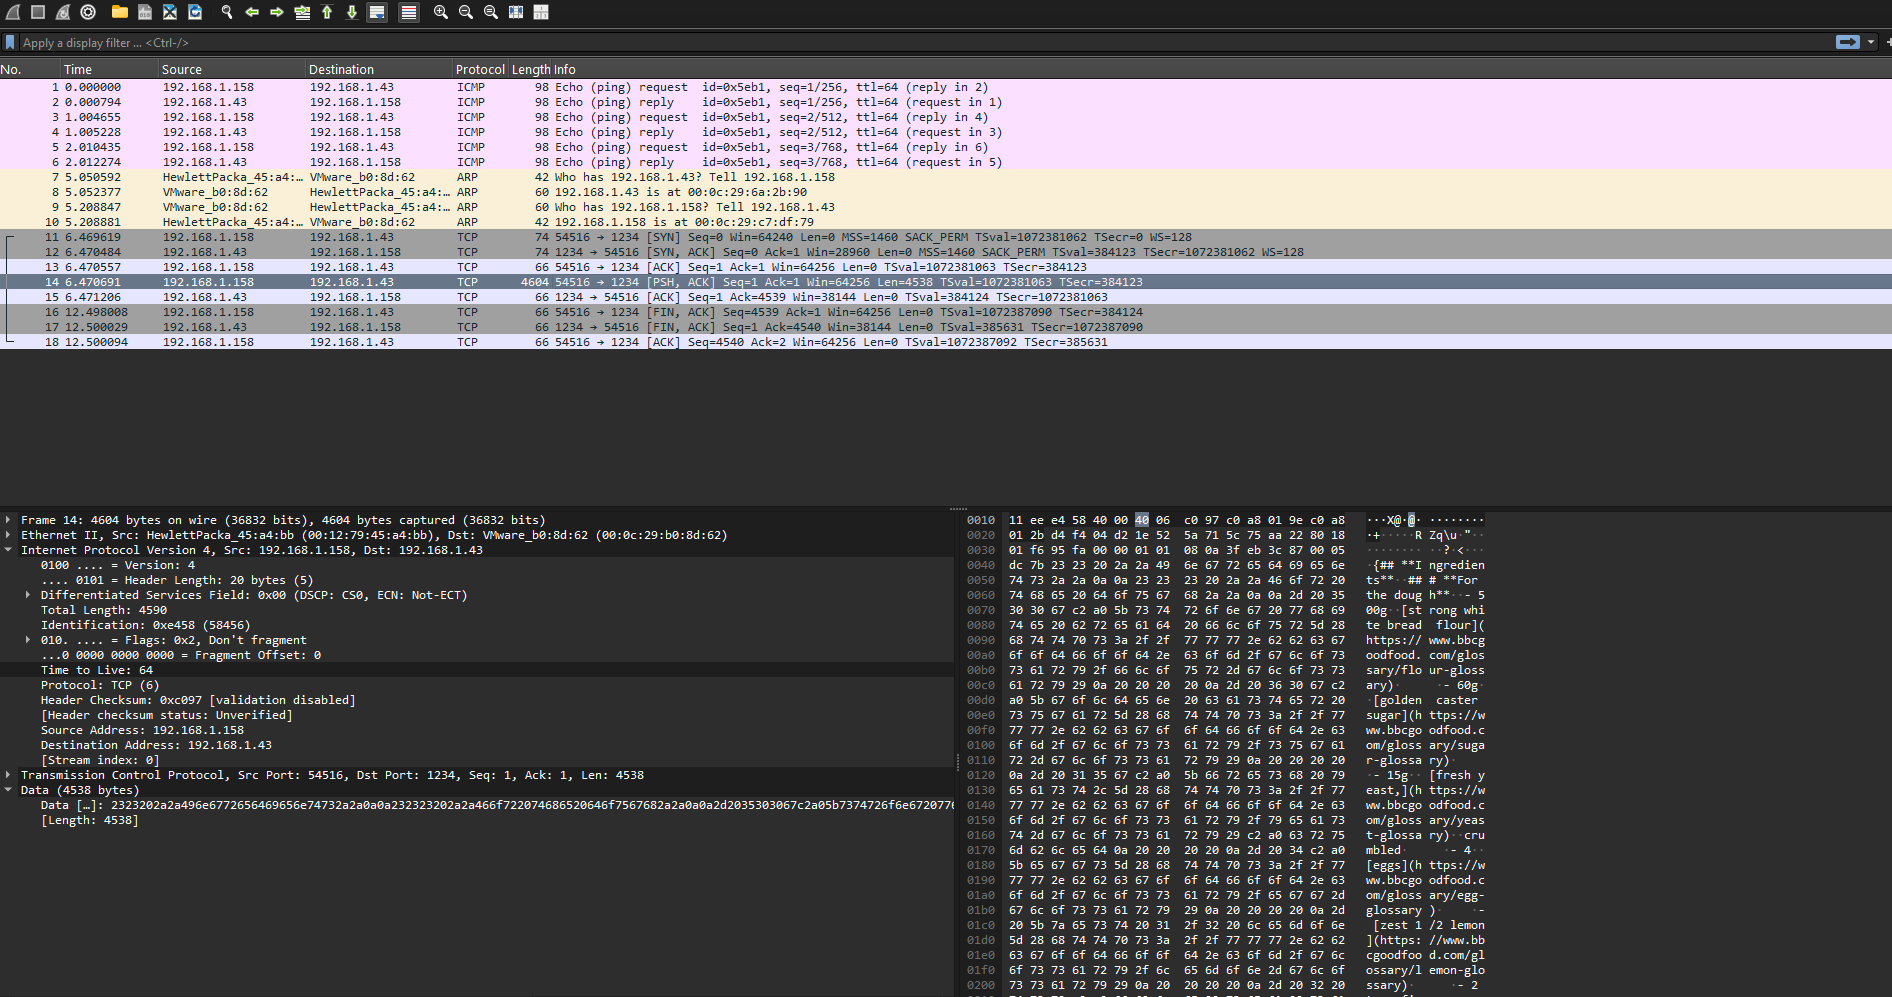
\includegraphics[width=0.95\textwidth]{images/Network_Analysis/ExhibitD_pcap.png}
    \caption{TCP data transfer of recipe information (Exhibit D)}
    \label{fig:exhibit_d_recipe}
\end{figure}

Frame 14 (timestamp 6.470691) in Exhibit D contained definitive evidence of recipe transmission:

\begin{itemize}
    \item 4538-byte payload from Smith's computer to the unknown laptop
    \item TCP [PSH, ACK] flags indicating immediate data delivery
    \item Content analysis revealed complete recipe text including:
        \begin{itemize}
            \item Ingredient list with precise measurements
            \item Preparation instructions with specific temperatures
            \item Proprietary techniques matching Lard\&land's "Honey Duff Donuts"
        \end{itemize}
\end{itemize}

This packet provides direct evidence of recipe exfiltration, answering investigation questions regarding both recipe theft and network activity.

\section{Travel and Steganography Evidence (Exhibit E)}

\subsection{Hawaii Travel Confirmation}
Frame analysis of Exhibit E revealed explicit evidence of planned travel to Hawaii:

\begin{figure}[htbp]
    \centering
    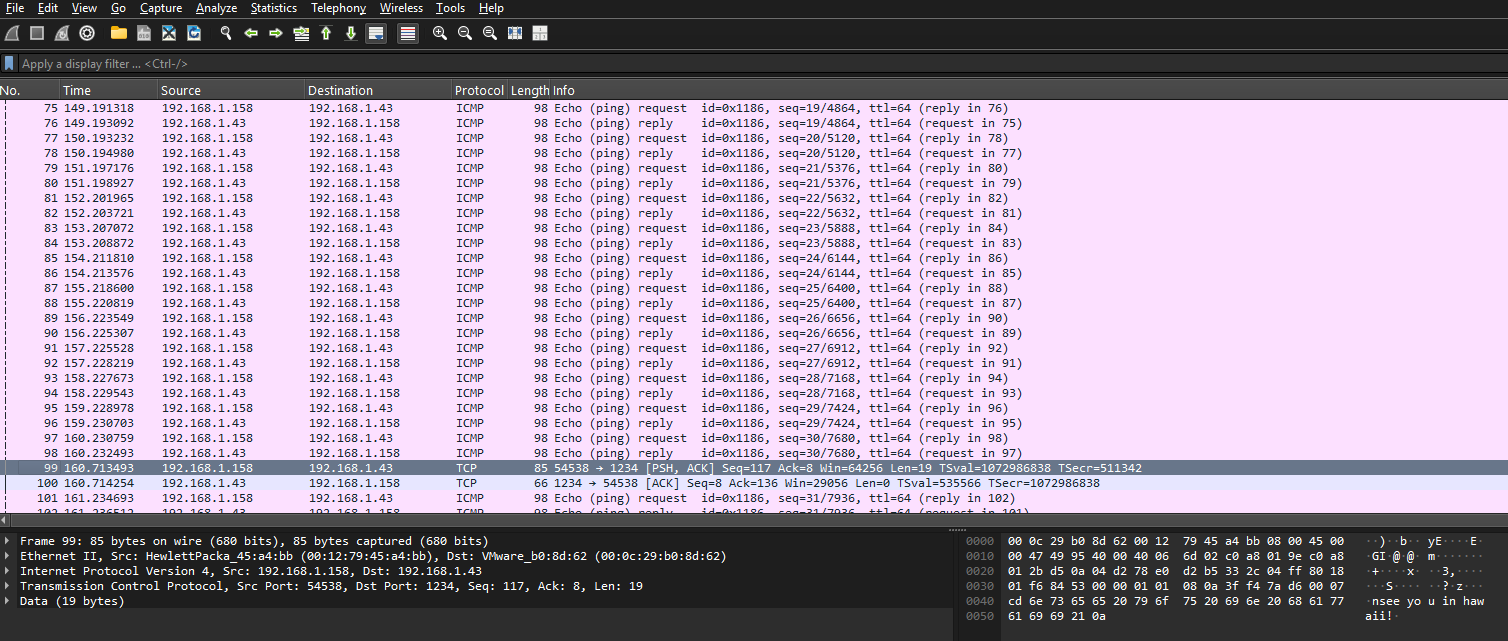
\includegraphics[width=0.95\textwidth]{images/Network_Analysis/ExhibitE_pcap_hawaii.png}
    \caption{Message confirming meeting in Hawaii (Exhibit E)}
    \label{fig:exhibit_e_hawaii}
\end{figure}

The message "see you in hawaii!" (timestamp 160.713493) provides:
\begin{itemize}
    \item Direct confirmation of Hawaii as destination
    \item Corroboration of the flight plan recovered from unallocated space
    \item Evidence of pre-arranged meeting following data transfer
\end{itemize}

\subsection{Steganography Usage Confirmation}
A second critical message in Exhibit E provided explicit admission of steganographic techniques:

\begin{figure}[htbp]
    \centering
    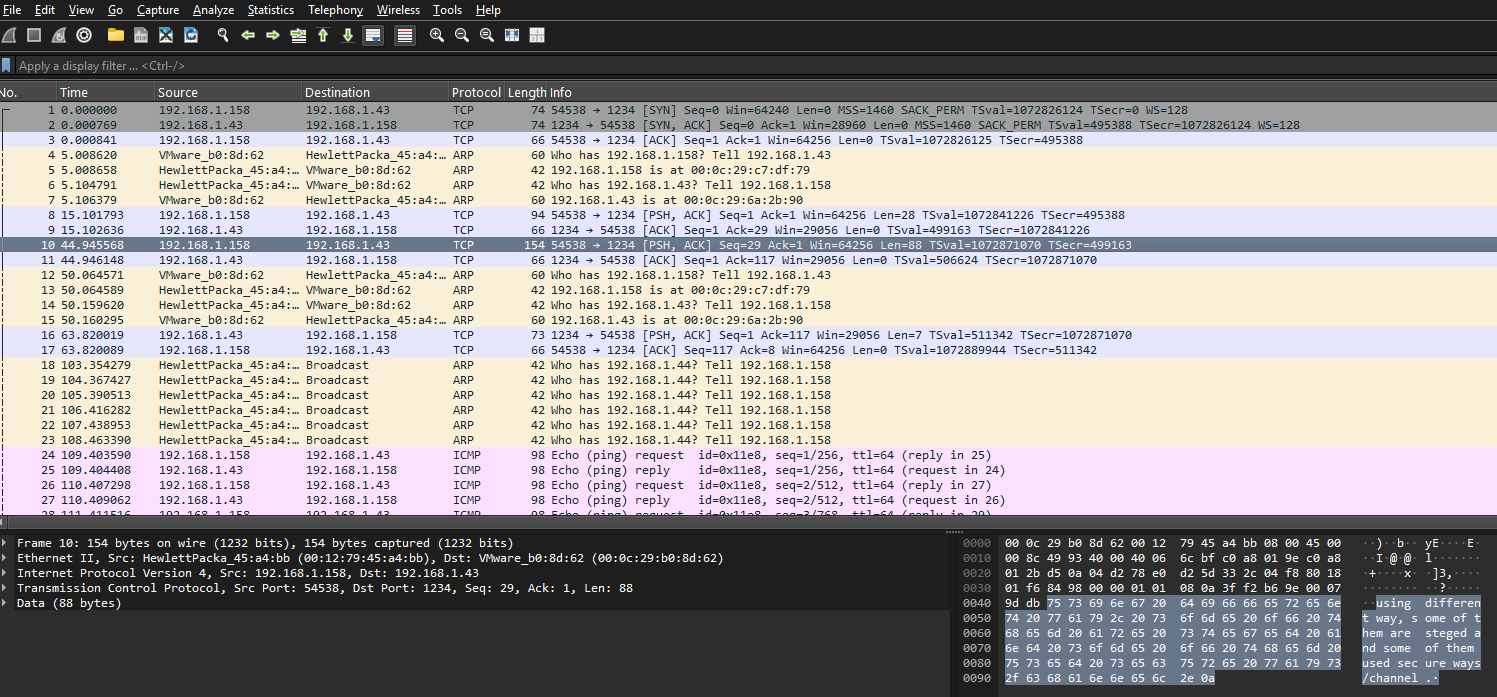
\includegraphics[width=0.95\textwidth]{images/Network_Analysis/ExhibitE_pcap_steg.png}
    \caption{Explicit reference to steganography usage (Exhibit E)}
    \label{fig:exhibit_e_steg}
\end{figure}

The message "using different way, some of them are steged and some of them used secure ways/channel" confirms:
\begin{itemize}
    \item Intentional use of steganography ("steged") for data concealment
    \item Implementation of multiple transfer methods for redundancy
    \item Technical knowledge of advanced data-hiding techniques
\end{itemize}

This communication directly corroborates the steganographic findings from the image analysis, establishing a consistent pattern of deliberate concealment across multiple evidence sources.

\section{Technical Communication Analysis}
Communication patterns across all packet captures revealed sophisticated operational security measures:

\begin{itemize}
    \item \textbf{Evasion Techniques}: Non-standard port usage (1234), virtualization technology, minimal session duration
    \item \textbf{Transmission Sequence}: ICMP connectivity testing → TCP session establishment → Data transfer → Acknowledgment → Follow-up planning
    \item \textbf{Technical Indicators}: TCP PSH flags for immediate delivery, calculated payload size, protocol manipulation
\end{itemize}

The chronological sequence of communications demonstrates methodical planning:
\begin{enumerate}
    \item Initial connectivity verification
    \item Recipe transmission (4538-byte payload)
    \item File transfer confirmation ("I have sent you a few files")
    \item Steganography acknowledgment 
    \item Hawaii travel arrangement
\end{enumerate}

This network evidence provides direct documentation of recipe data exfiltration, confirms Hawaii as Taurus Smith's planned destination, and validates the steganographic techniques identified elsewhere in the investigation.